\section{Experiments}
We did five dumps of the memory;
  \subsection{Clean dump}
  The first dump we did was right after boot, with factory settings and nothing done to the device 
  other than transferring the LiME LKM to the SD-card.
  
    The reason for this dump so we could see if we had set up our environment 
correctly and could read memory of the phone. The dump was also great for use 
when comparing to later dumps where we could see differences from a system with 
no significant use and compare them to the other experiments.

  \paragraph{Strings}

  \paragraph{Volatility}
  With volatility and its plugins we where able to see the process list
  \footnote{\url{https://github.com/volatilityfoundation/volatility/wiki/Linux\%20Command\%20Reference\#linux\_pslist}} 
  and other use full information about the system.

  \paragraph{PhotoRec}
  This program managed to get alot of files, such as java code files and txt 
  files containing information from internal logfiles as syslog (dmesg). It also 
  recovered some png files with pictures used by the Android launcher.
  
  \subsection{Pastebin entry}
  The second dump we did was after creating a pastebin entry on pastebin.com using 
  the stock Android browser (for 4.2.2),
  to see if we could find our entry in the memory.
  
  
  When starting to analyze this dump, we first started with the most basic. 
  Strings and hex editor; by searching for "pastebin.com". Other findings in this 
  process included a "timeline" on how the user got to the page patebin.com by 
  examining the memory segments before the hit on our string.

  \paragraph{Hex editor}
  This gave us a good way to examine the dump at its lowest level, by searching for 
  "p.a.s.t.e.b.i.n...c.o.m" we found the url we posted in our emulator

  \paragraph{Strings}
  Strings would show alot of results since there are often many hits on readable 
  data in these kind of dumps, by piping the output to grep we where able to 
  filter out text we wanted. Simply searching for pastebin.com we where able to 
  find the page it was posted on. 
  %Fant vi teksten som var skrevet også? brukte vi vol til dette? (yarascan) => Ja. Fant den også med strings/hex
  
  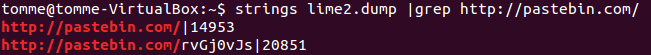
\includegraphics[scale=0.5]{strings_grep_pastebin.png}
  
  \subsection{Standard Text Message}
  The next dump was after sending a text message to the standard messages application. 
  Since the emulator provides an telnet interface, we where able to send a message 
  using \texttt{sms send <phoneNumber> <textMessage>}.
  
  This experiment was to see if it was possible to get recently received text 
  messages from a live system for use in a forensic environment.

  \paragraph{Strings}
  Same as above %?
  \subsection{Secure Text Message}
  Next we did the same as above, but after installing 
  TextSecure\footnote{\url{https://play.google.com/store/apps/details?id=org.thoughtcrime.securesms}}, 
  which encrypts the messages in a database. TextSecure was chosen since its a commonly 
  used application for securing your text 
  messages in transit (both sender and receiver would need to have it installed) and open source 
  so we could get a better understanding 
  on how it works. 
  
  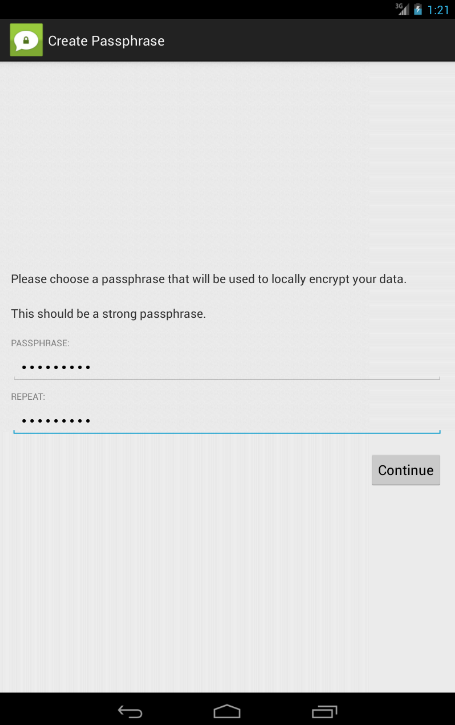
\includegraphics[scale=0.5]{textsecure.png}
  
  In some cases the device might have used anti-forensic tools to hide their 
  activity, we wanted to look into what information a memory analysis could 
  retrieve.
  \subsection{Screen lock}
  We also did a memory dump after creating a screen lock with a PIN code and using a passphrase.
  
  If the device has a unlocked bootloader it would often be possible to use out 
  method to retrieve memory of a device without wiping off all data from the 
  device. This experiment was done to see if we could find a passphrase or 
  incode from the memory dump.

  \paragraph{Strings}
  By searching for the pincode and passphrase we saw a pattern 
  %mer info om dette, var noe tekst etter koden som var lik  elns.
  \\
  \\
  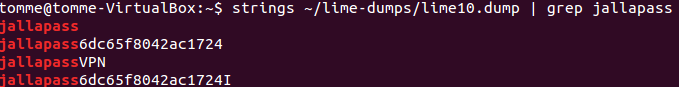
\includegraphics[scale=0.5]{strings_grep_pass.png}\\
  \\
  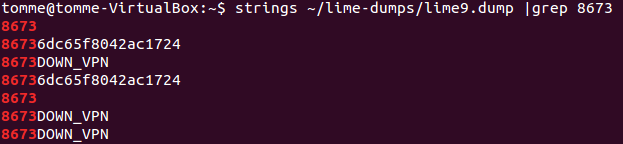
\includegraphics[scale=0.5]{strings_grep_pin.png}
